\documentclass[12pt]{article}

\usepackage{amsmath, mathtools}
\usepackage{amsfonts}
\usepackage{amssymb}
\usepackage{graphicx}
\usepackage{colortbl}
\usepackage{xr}
\usepackage{hyperref}
\usepackage{longtable}
\usepackage{xfrac}
\usepackage{tabularx}
\usepackage{float}
\usepackage{siunitx}
\usepackage{booktabs}
\usepackage{caption}
\usepackage{pdflscape}
\usepackage{afterpage}
\usepackage{braket}

\usepackage[round]{natbib}

%\usepackage{refcheck}

\hypersetup{
    bookmarks=true,         % show bookmarks bar?
      colorlinks=true,       % false: boxed links; true: colored links
    linkcolor=red,          % color of internal links (change box color with linkbordercolor)
    citecolor=green,        % color of links to bibliography
    filecolor=magenta,      % color of file links
    urlcolor=cyan           % color of external links
}

%% Comments

\usepackage{color}

\newif\ifcomments\commentstrue

\ifcomments
\newcommand{\authornote}[3]{\textcolor{#1}{[#3 ---#2]}}
\newcommand{\todo}[1]{\textcolor{red}{[TODO: #1]}}
\else
\newcommand{\authornote}[3]{}
\newcommand{\todo}[1]{}
\fi

\newcommand{\wss}[1]{\authornote{blue}{SS}{#1}} 
\newcommand{\plt}[1]{\authornote{magenta}{TPLT}{#1}} %For explanation of the template
\newcommand{\an}[1]{\authornote{cyan}{Author}{#1}}

%% Common Parts

\newcommand{\progname}{ProgName} % PUT YOUR PROGRAM NAME HERE %Every program
                                % should have a name


% For easy change of table widths
\newcommand{\colZwidth}{1.0\textwidth}
\newcommand{\colAwidth}{0.13\textwidth}
\newcommand{\colBwidth}{0.82\textwidth}
\newcommand{\colCwidth}{0.1\textwidth}
\newcommand{\colDwidth}{0.05\textwidth}
\newcommand{\colEwidth}{0.8\textwidth}
\newcommand{\colFwidth}{0.17\textwidth}
\newcommand{\colGwidth}{0.5\textwidth}
\newcommand{\colHwidth}{0.28\textwidth}

% Used so that cross-references have a meaningful prefix
\newcounter{defnum} %Definition Number
\newcommand{\dthedefnum}{GD\thedefnum}
\newcommand{\dref}[1]{GD\ref{#1}}
\newcounter{datadefnum} %Datadefinition Number
\newcommand{\ddthedatadefnum}{DD\thedatadefnum}
\newcommand{\ddref}[1]{DD\ref{#1}}
\newcounter{theorynum} %Theory Number
\newcommand{\tthetheorynum}{T\thetheorynum}
\newcommand{\tref}[1]{T\ref{#1}}
\newcounter{tablenum} %Table Number
\newcommand{\tbthetablenum}{T\thetablenum}
\newcommand{\tbref}[1]{TB\ref{#1}}
\newcounter{assumpnum} %Assumption Number
\newcommand{\atheassumpnum}{P\theassumpnum}
\newcommand{\aref}[1]{A\ref{#1}}
\newcounter{goalnum} %Goal Number
\newcommand{\gthegoalnum}{P\thegoalnum}
\newcommand{\gsref}[1]{GS\ref{#1}}
\newcounter{instnum} %Instance Number
\newcommand{\itheinstnum}{IM\theinstnum}
\newcommand{\iref}[1]{IM\ref{#1}}
\newcounter{reqnum} %Requirement Number
\newcommand{\rthereqnum}{P\thereqnum}
\newcommand{\rref}[1]{R\ref{#1}}
\newcounter{lcnum} %Likely change number
\newcommand{\lthelcnum}{LC\thelcnum}
\newcommand{\lcref}[1]{LC\ref{#1}}

\usepackage{fullpage}

\begin{document}

\title{Software Requirements Specification for Equation-of-motion methods: A 
set of tools for implementing and solving EOMs} 
\author{Gabriela S\'anchez D\'iaz}
\date{\today}
	
\maketitle

~\newpage

\pagenumbering{roman}

\tableofcontents

~\newpage

\section*{Revision History}

\begin{tabularx}{\textwidth}{p{3cm}p{2cm}X}
\toprule {\bf Date} & {\bf Version} & {\bf Notes}\\
\midrule
08-10-2020 & 1.0 & Creation of SRS \\
21-10-2020 & 1.1 & Address issues \#5, \#7 and \#8 regarding package name 
abbreviation 
and Traceability matrices section.\\
%Date 2 & 1.1 & Notes\\
\bottomrule
\end{tabularx}

~\newpage

\section{Reference Material}

This section records information for easy reference.

\subsection{Table of Units}

Throughout this document SI (Syst\`{e}me International d'Unit\'{e}s) is employed
as the unit system.  In addition to the basic units, several derived units are
used as described below.  For each unit, the symbol is given followed by a
description of the unit and the SI name.
~\newline

\renewcommand{\arraystretch}{1.2}
%\begin{table}[ht]
  \noindent \begin{tabular}{l l l} 
    \toprule		
    \textbf{symbol} & \textbf{unit} & \textbf{SI}\\
    \midrule 
    \si{\metre} & length & metre\\
%    \si{\kilogram} & mass	& kilogram\\
%    \si{\second} & time & second\\
%    \si{\celsius} & temperature & centigrade\\
    \si{\joule} & energy & joule\\
%    \si{\watt} & power & watt (W = \si{\joule\per\second})\\
    \bottomrule
  \end{tabular}
  %	\caption{Provide a caption}
%\end{table}

%\plt{Only include the units that your SRS actually uses.}

%\plt{Derived units, like newtons, pascal, etc, should show their derivation
 %   (the units they are derived from) if their constituent units are in the
  %  table of units (that is, if the units they are derived from are used in the
   % document).  For instance, the derivation of pascals as
   % $\si{\pascal}=\si{\newton\per\square\meter}$ is shown if newtons and m are
   % both in the table.  The derivations of newtons would not be shown if kg and
   % s are not both in the table.}

%\plt{The symbol for units named after people use capital letters, but the name
 % of the unit itself uses lower case.  For instance, pascals use the symbol Pa,
 % watts use the symbol W, teslas use the symbol T, newtons use the symbol N,
  %etc.  The one exception to this is degree Celsius.  Details on writing metric
  %units can be found on the 
  %\href{https://www.nist.gov/pml/weights-and-measures/writing-metric-units}
  %{NIST} web-page.}

\subsection{Table of Symbols}

The table that follows summarizes the symbols used in this document along with
their units. 
% The symbols are listed in alphabetical order.

\renewcommand{\arraystretch}{1.2}
%\noindent \begin{tabularx}{1.0\textwidth}{l l X}
\noindent \begin{longtable*}{l l p{12cm}} \toprule
\textbf{symbol} & \textbf{unit} & \textbf{description}\\
\midrule 
%$A_C$ & \si[per-mode=symbol] {\square\metre} & coil surface area
%\\
%$A_\text{in}$ & \si[per-mode=symbol] {\square\metre} & surface area over 
%which heat is transferred in
%\\
$n$ & unitless & number of spinorbitals in the basis set\\
$N$ & unitless & number of electrons in a system\\
%$\{\phi_i|i=1,2,.,n\}$ & $\si{\metre}^{-3/2}$ & spinorbital basis set\\
$\phi_p$ & $\si{\metre}^{-3/2}$ & p-th spinorbital of the basis set, 
can also be represented as p\\
$\hat{a}_p$ & unitless & Second-quantization anihilation operator for 
spinorbital p\\ 
$\hat{a}^\dagger_p$ & unitless & Second-quantization creation operator for 
spinorbital p\\ 
$\delta_{ij}$ & unitless & Kronecker delta function (1 for i=j, 0 otherwise)\\
$\mathbf{I}$ & unitless & Identity matrix, its elements are $\delta_{ij}$\\
$\Psi^{N}$ & $\si{\metre}^{-3/2}$ & N-electron stationary state wavefunction\\
$\ket{\Psi^{(N)}_0}$ & $\si{\metre}^{-3/2}$ & N-electron ground state 
wavefunction (vector representation using Dirack's bra-ket notation)\\
$\ket{\Psi^{(N \pm K)}_n}$ & $\si{\metre}^{-3/2}$ & (N $\pm$ K)-electron, n-th 
excited state wavefunction (vector representation using Dirack's bra-ket 
notation)\\
$\hat{H}$ & \si{\joule} & Hamiltonian operator\\
$\hat{Q}$ & unitless & Transition operator\\
$\hat{Q}^{\dagger}$ & unitless & Conjugate transpose of $\hat{Q}$\\
$\hat{Q}^{\pm K}_{k}$ & unitless & $\hat{Q}$ of the 
(N$\pm$K)-stationary state $k$ (relative to the N-electron reference 
stationary state)\\
$\hat{h}$ & \si{\joule} & 1-electron Hamiltonian operator\\
$\mathbf{h}$ & \si{\joule} & 1-electron integral matrix\\
$h_{pq}$ & \si{\joule} & p,q-th element of $\mathbf{h}$\\
$\hat{v}$ & \si{\joule} & 2-electron Hamiltonian operator\\
$\mathbf{v}$ & \si{\joule} & 2-electron integral matrix\\
$v_{pqrs}$ & \si{\joule} & the p,q,r,s-th element of $\mathbf{v}$\\
$E$ & \si{\joule} & energy\\
$\Delta E_{k}$ & \si{\joule} & energy difference between two stationary 
states ($k$ and the reference one)\\
$\boldsymbol{\gamma}$ & unitless& 1-electron reduced density matrix\\
$\gamma_{pq}$ & unitless& p,q-th element of $\boldsymbol{\gamma}$\\
$\gamma_{pq}$ & unitless& p,q-th element of $\boldsymbol{\gamma}$\\
$\Gamma_{pqrs}$ & unitless& p,q,r,s-th element of $\boldsymbol{\Gamma}$\\
$\gamma_{m;0k}$ & unitless& m-th element of the transition density matrix 
between states $\ket{\Psi^{(N)}_0}$ and $\ket{\Psi^{(N \pm K)}_{k}}$\\
$p,q,r,s$ & unitless & arbitrary spinorbital index\\
$\mathbf{r}$ & \si{\metre} & Electronic coordinates\\
$\mathbf{R}$ & \si{\metre} & Nuclear coordinates\\
\bottomrule
\end{longtable*}
%\plt{Use your problems actual symbols.  The si package is a good idea to use 
%for units.}
\subsection{Notation}
The symbols and notation used through this document are consistent with the 
quantum chemistry literature and with existing documentation for 
equation-of-motion methods (see, e.g., \cite{Pernal2018}, \cite{McKoy1977} and 
Chapters 1 nad 2 of \cite{szabo-ostlund}). Some examples of this notation are: 
the operator of an observable O is denoted by $\hat{O}$, Dirac's bra-ket 
notation ($\bra{}$ $\ket{}$) is used for the representation of a state's wave 
function and vector or matrix parameters are indicated with bold face (like the 
identity matrix in the table above).


\subsection{Abbreviations and Acronyms}

\renewcommand{\arraystretch}{1.2}
\begin{tabular}{l l} 
  \toprule		
  \textbf{symbol} & \textbf{description}\\
  \midrule 
  A & Assumption\\
  BS & Basis set(s)\\
  DD & Data Definition\\
  EA & Electron affinity\\
  EOMEE& Equation-of-motion for excited states\\
  GD & General Definition\\
  GS & Goal Statement\\
  IM & Instance Model\\
  IP & Ionization Potential\\
  LC & Likely Change\\
  MO & Molecular orbital\\
  PS & Physical System Description\\
  PC & Personal Computer\\
  QC & Quantum chemistry\\
  R & Requirement\\
  SRS & Software Requirements Specification\\
  RDM & Reduced density matrix\\
  T & Theoretical Model\\
  TDM & Transition density matrix\\
  \bottomrule
\end{tabular}\\

%\plt{Add any oher abbreviations or acronyms that you add}

\newpage

\pagenumbering{arabic}

%\plt{This SRS template is based on \citet{SmithAndLai2005, SmithEtAl2007}.  It
 % will get you started.  You should not modify the section headings, without
  %first discussing the change with the course instructor.  Modification means
 % you are not following the template, which loses some of the advantage of a
  %template, especially standardization.  Although the bits shown below do not
  %include type information, you may need to add this information for your
  %problem.  If you are unsure, please can ask the instructor.}

%\plt{Feel free to change the appearance of the report by modifying the LaTeX
 % commands.}

%\plt{This template document assumes that a single program is being documented.
 % If you are documenting a family of models, you should start with a commonality
  %analysis.  A separate template is provided for this.  For program
  %families you should look at \cite{Smith2006, SmithMcCutchanAndCarette2017}.
  %Single family member programs are often programs based on a single physical
  %model.  General purpose tools are usually documented as a family.  Families of
  %physical models also come up.}

%\plt{The SRS is not generally written, or read, sequentially.  The SRS is a
 % reference document.  It is generally read in an ad hoc order, as the need
  %arises.  For writing an SRS, and for reading one for the first time, the
  %suggested order of sections is:
%\begin{itemize}
%\item Goal Statement
%\item Instance Models
%\item Requirements
%\item Introduction
%\item Specific System Description
%\end{itemize}
%}

%\plt{Guiding principles for the SRS document:
%\begin{itemize}
%\item Do not repeat the same information at the same abstraction level.  If
 % information is repeated, the repetition should be at a different abstraction
  %level.  For instance, there will be overlap between the scope section and the
  %assumptions, but the scope section will not go into as much detail as the
  %assumptions section.
%\end{itemize}
%}

%\plt{The template description comments should be disabled before submitting this
 % document for grading.}

%\plt{You can borrow any wording from the text given in the template.  It is part
 % of the template, and not considered an instance of academic integrity.  Of
  %course, you need to cite the source of the template.}

%\plt{When the documentation is done, it should be possible to trace back to the
 % source of every piece of information.  Some information will come from
  %external sources, like terminology.  Other information will be derived, like
  %General Definitions.}

%\plt{An SRS document should have the following qualities: unambiguous,
 % consistent, complete, validatable, abstract and traceable.}

%\plt{The overall goal of the SRS is that someone that meets the Characteristics
 % of the Intended Reader (Section~\ref{sec_IntendedReader}) can learn,
 % understand and verify the captured domain knowledge.  They should not have to
  %trust the authors of the SRS on any statements.  They should be able to
  %independently verify/derive every statement made.}

\section{Introduction}

%\plt{The introduction section is written to introduce the problem.  It starts
%  general and focuses on the problem domain. The general advice is to start 
%with
%a paragraph or two that describes the problem, followed by a ``roadmap''
%paragraph.  A roadmap orients the reader by telling them what sub-sections to
%expect in the Introduction section.}

The spectroscopic characterization of atomic and molecular systems is one 
of the fundamental techniques in the fields related to Chemistry. \\
%\an{Agregar figura con un espectro UV y su molécula, explicar que el espectro 
%es el resultado de la transicion de la molecula del estado estacionario base 
%$\Psi_0$ al esxcitado $\Psi_1$. Agregar los diagramas de la TOM 
%correspondientes aclarando que estos son una representacion valida de $\Psi_0$ 
%y $\Psi_1$ si estos estados son predominantemente monoconfiguracionales. 
%Alternativamente agregar solo un esquema de las energias relativas de ambos 
%estados y el delta de energia entre ellos que seria lo que EOM va a calcular.}
As part of 
the methods developed in computational quantum chemistry, Equation-of-motion 
(EOM) methods offer an alternative approach to the prediction of molecular 
properties such as excitation energies, ionization potentials or electron 
affinities by directly targeting the evaluation of these magnitudes.\\ 
The present document introduces the requirements description for the 
development of a set of tools for implementing and solving EOM 
equations (package name: Equation-of-motion for excited states, abbreviated as 
EOMEE). The formatting of this document will follow the SRS templates 
introduced 
by 
\cite{Smith2016} and \cite{SmithEtAl2007}.


\subsection{Purpose of Document}

%\plt{This section summarizes the purpose of the SRS document.  It does not focus
  %on the problem itself.  The problem is described in the ``Problem
  %Description'' section (Section~\ref{Sec_pd}).  The purpose is for the document
  %in the context of the project itself, not in the context of the CAS 741
  %course.  Although the ``purpose'' of the document is to get a grade in 741,
  %you should not mention this.  Instead, ``fake it'' as if this is a real
 % project.  The purpose section will be similar between projects.  The purpose
 % of the document is the purpose of the SRS, including communication, planning
%  for the design stage, etc.}

%\an{
	This document intends to establish the parameters under which the quality 
	of the program EOMEE can be assessed %(correctness: what the code should 
	%do; 
%reusability; performance)
%}  

\subsection{Scope of Requirements} 

%\plt{Modelling the real world requires simplification.  The full complexity of
%  the actual physics, chemistry, biology is too much for existing models, and
%  for existing computational solution techniques.  Rather than say what is in
%  the scope, it is usually easier to say what is not.  You can think of it as
%  the scope is initially everything, and then it is constrained to create the
%  actual scope.  For instance, the problem can be restricted to 2 dimensions, 
%or
%  it can ignore the effect of temperature (or pressure) on the material
%  properties, etc.}  
%
%\plt{The scope section is related to the assumptions section
%  (Section~\ref{sec_assumpt}).  However, the scope and the assumptions are not
%  at the same level of abstraction.  The scope is at a high level.  The focus 
%is
%  on the ``big picture'' assumptions.  The assumptions section lists, and
%  describes, all of the assumptions.}

EOMEE will evaluate the energy variations in processes that involve up to two 
particle transitions. In a standard PC its applicability will be limited to 
molecular systems with about 60 molecular orbital (MO) basis due to the demands 
of memory resources.

\subsection{Characteristics of Intended Reader} \label{sec_IntendedReader}

%\plt{This section summarizes the skills and knowledge of the readers of the
%  SRS.  It does NOT have the same purpose as the ``User Characteristics''
%  section (Section~\ref{SecUserCharacteristics}).  The intended readers are the
%  people that will read, review and maintain the SRS.  They are the people that
%  will conceivably design the software that is intended to meet the
%  requirements.  The user, on the other hand, is the person that uses the
%  software that is built.  They may never read this SRS document.  Of course,
%  the same person could be a ``user'' and an ``intended reader.''}
%
%\plt{The intended reader characteristics should be written as unambiguously and
%  as specifically as possible.  Rather than say, the user should have an
%  understanding of physics, say what kind of physics and at what level.  For
%  instance, is high school physics adequate, or should the reader have had a
%  graduate course on advanced quantum mechanics?}

The reader of this document must have a Level-1 undergraduate knowledge of 
mathematics 
(specifically of linear algebra), and quantum chemistry or physics. 
Additionally, familiarity with the formalism of second-quantization and some 
programming skills are required.

\subsection{Organization of Document}

%\plt{This section provides a roadmap of the SRS document.  It will help the
 % reader orient themselves.  It will provide direction that will help them
  %select which sections they want to read, and in what order.  This section will
  %be similar between project.}
%\an{
	The outline of the document is as follows: In section 3 the context of the 
systems, its constraints and characteristics of the user are described. Section 
4 deepens the description by providing information of the intended inputs and 
outputs, the mathematical models that characterize the physical problem and the 
assumptions being made. Section (4) lists the system's functional and 
nonfunctional requirements. The expected changes, and the invariable ones are 
stated in sections 5 and 6, respectively. Finally, section 7 shows the 
traceability matrices and graphs and section 8 lists the values of auxiliary 
constants.
%}

\section{General System Description}

This section provides general information about the system.  It identifies the
interfaces between the system and its environment, describes the user
characteristics and lists the system constraints. 
% \plt{This text can likely be
%  borrowed verbatim.}
%
%\plt{The purpose of this section is to provide general information about the
%  system so the specific requirements in the next section will be easier to
%  understand. The general system description section is designed to be
%  changeable independent of changes to the functional requirements documented 
%in
%  the specific system description. The general system description provides a
%  context for a family of related models.  The general description can stay the
%  same, while specific details are changed between family members.}

\subsection{System Context}

%\plt{Your system context will include a figure that shows the abstract view of
% the software.  Often in a scientific context, the program can be viewed
%abstractly following the design pattern of Inputs $\rightarrow$ Calculations
%$\rightarrow$ Outputs.  The system context will therefore often follow this
%pattern.  The user provides inputs, the system does the calculations, and then
%provides the outputs to the user.  The figure should not show all of the
%inputs, just an abstract view of the main categories of inputs (like material
%properties, geometry, etc.).  Likewise, the outputs should be presented from
%an abstract point of view.  In some cases the diagram will show other external
%entities, besides the user.  For instance, when the software product is a
%library, the user will be another software program, not an actual end user.}

Figure \ref{Fig_SystemContext} describes EOMEE's context. 
External interactions are indicated by circles, and the program by a rectangle 
area. Information pertinent to the input and output data are indicated at the 
left and right of the program.
%User---1 and 2-electron integrlas, 1 and 2 RDMs---eomee--- energies, TDMs

The user will submit the programs arguments (1- and 2-electron integrals, 1- 
and 2-electron reduced density matrices (RDMs)); then EOMEE will process
that information and return the resulting transition density matrices (TDMs). 

\begin{figure}[h!]
	\begin{center}
		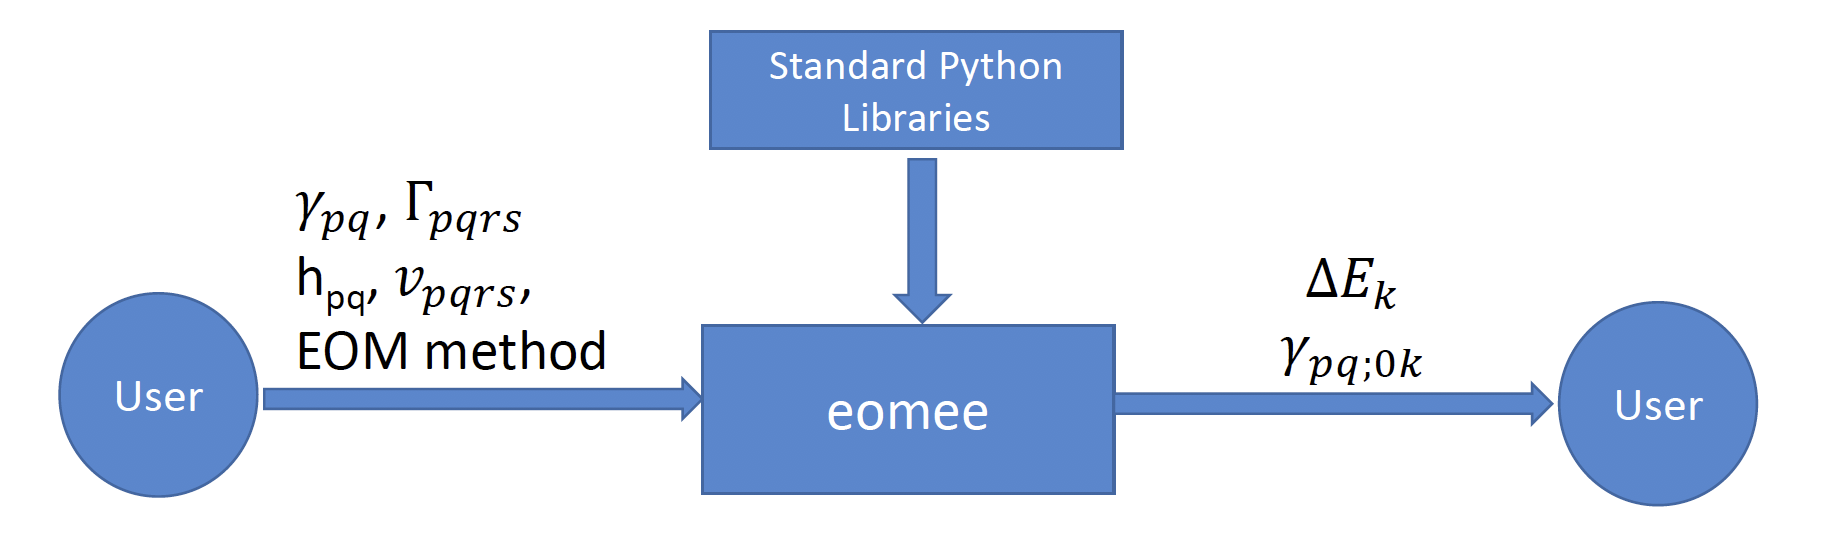
\includegraphics[width=0.6\textwidth]{GlobalStatement}
		\caption{eomee Context}
		\label{Fig_SystemContext} 
	\end{center}
\end{figure}

%\plt{For each of the entities in the system context diagram its responsibilities
% should be listed.  Whenever possible the system should check for data quality,
%  but for some cases the user will need to assume that responsibility.}

\begin{itemize}
	\item User Responsibilities:
	\begin{itemize}
		\item Provide the inputs for the atomic or molecular system of interest.
		\item Guarantee that enough memory resources are available for the intended 
		study system.
		\item Verify that the output data has physical meaning for his intended system.
	\end{itemize}
	\item EOMEE Responsibilities:
	\begin{itemize}
		\item Detect data type mismatch, such as a string of characters 
		instead of an array.
		\item Detect data value mismatch, such as incorrect dimensions of input arrays.
		\item Verify that the input matrices have the correct symmetries.
		\item Transform the electron integrals and RDMs from the MO to the spinorbital 
		representation.
		\item Evaluate the transition energies and density matrices for the user 
		selected EOM method.
	\end{itemize}
\end{itemize}

\subsection{User Characteristics} \label{SecUserCharacteristics}

%\plt{This section summarizes the knowledge/skills expected of the user.
%  Measuring usability, which is often a required non-function requirement,
%  requires knowledge of a typical user.  As mentioned above, the user is a
%  different role from the ``intended reader,'' as given in
%  Section~\ref{sec_IntendedReader}.  As in Section~\ref{sec_IntendedReader}, 
%the
%  user characteristics should be specific an unambiguous.  For instance, ``The
%  end user of \progname{} should have an understanding of undergraduate Level 1
%  Calculus and Physics.''}

The user of EOMEE should have first-year undergraduate level of chemistry 
or physics so that she/he is familiar with the concepts of electronic 
excitation (or ionization) of an atomic or molecular system. To generate the 
program's input data, the user needs also experience in the field of 
computational an theoretical chemistry or physics.

\subsection{System Constraints}

%\plt{System constraints differ from other type of requirements because they
 % limit the developers’ options in the system design and they identify how the
 % eventual system must fit into the world. This is the only place in the SRS
  %where design decisions can be specified.  That is, the quality requirement for
  %abstraction is relaxed here.  However, system constraints should only be
  %included if they are truly required. In the context of CAS 741, you often will
  %may not have any system constraints.}

%\an{
	Availability of general Python libraries is required for the development 
of EOMEE.
%}

\section{Specific System Description}

This section first presents the problem description, which gives a high-level
view of the problem to be solved.  This is followed by the solution characteristics
specification, which presents the assumptions, theories, definitions and finally
the instance models.  
%\plt{Add any project specific details that are relevant for the section 
%overview.}

\subsection{Problem Description} \label{Sec_pd}

The development of EOMEE is motivated by the need to create a common framework 
for the solution of EOM methods based on the RDMs. This will allow the 
comparison between different wavefunction based approaches from computational 
quantum chemistry and serve as an intermediate point for the development of 
future scientific work based in the TDMs.\\

\subsubsection{Terminology and  Definitions}

%\plt{This section is expressed in words, not with equations.  It provide the
%  meaning of the different words and phrases used in the domain of the problem.
%The terminology is used to introduce concepts from the world outside of the
%mathematical model  The terminology provides a real world connection to give 
%the
%mathematical model meaning.}

This subsection provides a list of terms that are used in the subsequent
sections and their meaning, with the purpose of reducing ambiguity and making it
easier to correctly understand the requirements:

\begin{itemize}

\item \textbf{reference stationary state}: State onto which the excitation 
operator acts. Is usually taken as the lowest energy N-electron stationary 
state (ground 
state).
\item \textbf{excitation or transition operator}: Operator that transforms the 
reference N-electron stationary state into a different stationary state.
\item \textbf{excited state}: an stationary state other than the ground one. 
Higher in 
energy and potentially with a different number of electrons.
\item \textbf{electron density matrix}: matrix corresponding to the electron 
density distribution represented in the spinorbital basis set.
\item \textbf{spinorbital}: orthonormal function of the space and spin 
coordinates of a single electron.
\item \textbf{electron integrals}: energy contributions of the different 
interaction between the electrons and nuclei in the system.
\item \textbf{quantum chemistry methods}: methods that deal with solving the 
Schr\"odinger equation.

\end{itemize}

\subsubsection{Physical System Description} \label{sec_phySystDescrip}

%\plt{The purpose of this section is to clearly and unambiguously state the
%  physical system that is to be modelled. Effective problem solving requires a
%  logical and organized approach. The statements on the physical system to be
%  studied should cover enough information to solve the problem. The physical
%  description involves element identification, where elements are defined as
%  independent and separable items of the physical system. Some example elements
%  include acceleration due to gravity, the mass of an object, and the size and
%  shape of an object. Each element should be identified and labelled, with 
%their
%  interesting properties specified clearly. The physical description can also
%  include interactions of the elements, such as the following: i) the
%  interactions between the elements and their physical environment; ii) the
%  interactions between elements; and, iii) the initial or boundary conditions.}

The EOMEE's physical system includes the following elements:

\begin{itemize}

\item[PS1:] The N-electron reference stationary state $\Psi^{(N)}_0$, 
characterized by the 1- and 2-RDMs.

\item[PS2:] The $k$th excited state $\Psi^{(N \pm K)}_k$.

\item[PS3:] The excitation operator $\hat{Q}^{(N \pm K)}_k$ that transform 
$\Psi^{(N)}_0$ into $\Psi^{(N \pm K)}_k$.

\item[PS4:] The electronic Hamiltonian operator $\hat{H}$ which contains the 
information about the interactions between the particles in the system.

\end{itemize}

%\plt{A figure here makes sense for most SRS documents}

% \begin{figure}[h!]
% \begin{center}
% %\rotatebox{-90}
% {
%  \includegraphics[width=0.5\textwidth]{<FigureName>}
% }
% \caption{\label{<Label>} <Caption>}
% \end{center}
% \end{figure}

\subsubsection{Goal Statements}

\noindent Given the density matrices and the 1- and 2-electron integrals of a 
reference N-electron stationary state and an EOM method, the goal statements 
are:

\begin{itemize}

\item[GS\refstepcounter{goalnum}\thegoalnum \label{GS:energy}:] Determine the 
transition energies.
\item[GS\refstepcounter{goalnum}\thegoalnum \label{GS:tdms}:] Determine the 
transition density matrices.

\end{itemize}

\subsection{Solution Characteristics Specification}

The instance models that govern EOMEE are presented in
Subsection~\ref{sec_instance}.  The information to understand the meaning of the
instance models and their derivation is also presented, so that the instance
models can be verified.

\subsubsection{Assumptions} \label{sec_assumpt}

%\plt{The assumptions are a refinement of the scope.  The scope is general, 
%where
%  the assumptions are specific.  All assumptions should be listed, even those
%  that domain experts know so well that they are rarely (if ever) written 
%down.}
%\plt{The document should not take for granted that the reader knows which
%  assumptions have been made. In the case of unusual assumptions, it is
%  recommended that the documentation either include, or point to, an 
%explanation
%  and justification for the assumption.}

This section simplifies the original problem and helps in developing the
theoretical model by filling in the missing information for the physical
system. The numbers given in the square brackets refer to the theoretical model
[T], general definition [GD], data definition [DD], instance model [IM], or
likely change [LC], in which the respective assumption is used.

\begin{itemize}

%\item[A\refstepcounter{assumpnum}\theassumpnum \label{A_meaningfulLabel}:]
%  \plt{Short description of each assumption.  Each assumption
%    should have a meaningful label.  Use cross-references to identify the
%    appropriate traceability to T, GD, DD etc., using commands like dref, ddref
%    etc.  Each assumption should be atomic - that is, there should not be an
%    explicit (or implicit) ``and'' in the text of an assumption.}
\item[A\refstepcounter{assumpnum}\theassumpnum \label{A_transition_op_approx}:] 
The 
transition operator can be approximated by a finite expansion in 
second-quantization operators strings (BS). [~\dref{G_approxQ}]
\item[A\refstepcounter{assumpnum}\theassumpnum \label{A_dms_mointeg}:] The EOM 
methods can be expressed in terms of the 1- and 2-reduced density
matrices of the reference state and the 1- and 2-electron integrals.
[\iref{IM_IP}]-[\iref{IM_DEA}]
\item[A\refstepcounter{assumpnum}\theassumpnum \label{A_int_mos}:] The 1- and 
2-electron integrals are in the MO basis representation. [\ddref{D_oneints}], 
[\ddref{D_twoints}]
\item[A\refstepcounter{assumpnum}\theassumpnum \label{A_symmetry}:] The input 
electron integrals and RDMs have the correct symmetries.[\ddref{D_oneints}], 
[\ddref{D_twoints}], [\ddref{D_1rdm}], 
[\ddref{D_2rdm}]
\item[A\refstepcounter{assumpnum}\theassumpnum \label{A_killercond}:] The 
condition $\hat{Q}^{\dagger}\ket{\Psi^{N}_0} = 0$ (``killer condition") is 
fulfilled. [\dref{G_EOM}]
\item[A\refstepcounter{assumpnum}\theassumpnum \label{A_sproj}:] The EOM method 
is expressed as a determined system of equations by projecting onto the 
transition operator's BS. [\dref{G_EOM}], [\iref{IM_IP}]-[\iref{IM_DEA}]

\end{itemize}

\subsubsection{Theoretical Models}\label{sec_theoretical}

%\plt{Theoretical models are sets of abstract mathematical equations or axioms
%  for solving the problem described in Section ``Physical System Description''
%  (Section~\ref{sec_phySystDescrip}). Examples of theoretical models are
%  physical laws, constitutive equations, relevant conversion factors, etc.}

This section focuses on the general equations and laws that EOMEE is based on.

~\newline

\noindent
\begin{minipage}{\textwidth}
\renewcommand*{\arraystretch}{1.5}
\begin{tabular}{| p{\colAwidth} | p{\colBwidth}|}
  \hline
  \rowcolor[gray]{0.9}
  Number& T\refstepcounter{theorynum}\thetheorynum \label{T_SchrodingerEq}\\
  \hline
  Label&\bf Time-independent Schr\"odinger equation\\
  \hline
  Equation&  $\hat{H}\Psi^{(N)} = E \Psi^{(N)}$\\
  \hline
  Description & 
                The equation above represents the time-independent 
                nonrelativistic Schr\"odinger equation. Where $\hat{H}$ is the 
                Hamiltonian operator, $\Psi^{(N)}$, the N-electron stationary 
                state wavefunction, and ($E$) the corresponding total energy of 
                the system. Finding the solutions to this equation is the main 
                objective of quantum chemistry methods. \\
  \hline
  Source &  \cite{szabo-ostlund}
  \\
  \hline
  Ref.\ By & \dref{G_EOM}\\
  \hline
\end{tabular}
\end{minipage}\\
\newline
A more explicit representation of this equation includes its dependence on the 
nuclear and electronic coordinates of the particles composing the system 
($\textbf{R}$ and $\textbf{r}$ respectively):
$\hat{H}\Psi^{(N)}(\textbf{r,R}) = E_{Tot} \Psi^{(N)}(\textbf{r,R}) $\\
where $\hat{H}= \hat{T}_{nuc} + \hat{T}_{el} + \hat{V}_{nuc-nuc} + 
\hat{V}_{el-el} + \hat{V}_{nuc-el}$ includes the kinetic ($\hat{T}$) and 
potential ($\hat{V}$) energies of the electrons ($el$) and nuclei ($nuc$).\\
Because quantum chemical methods are generally applied under the 
Born-Oppenheimer approximation (which allows to separates the nuclear and 
electronic 
motions) the actual expression used through this document is:\\
$\hat{H}_{el}\Psi^{(N)}_{el}(\textbf{r,R}) = E_{el}(\textbf{R}) 
\Psi^{(N)}_{el}(\textbf{r,R})$\\
in which the term $\hat{T}_{nuc}$ in not included in the Hamiltonian operator. 
The coulombic interactions between the atoms ($\hat{V}_{nuc-nuc}$) become a 
constant factor for a given set of $\textbf{R}$ (molecular geometry), so that 
the electronic energy 
($E_{el}(\textbf{R})$) depends on these coordinates.\\
For notation simplicity we will drop the subscripts and use $\hat{H}\Psi^{(N)} 
= E \Psi^{(N)}$ as the electronic Schr\"odinger equation for an N-electron, 
M-atom system.
~\newline

\noindent
\begin{minipage}{\textwidth}
	\renewcommand*{\arraystretch}{1.5}
	\begin{tabular}{| p{\colAwidth} | p{\colBwidth}|}
		\hline
		\rowcolor[gray]{0.9}
		Number& T\refstepcounter{theorynum}\thetheorynum \label{T_ExcState}\\
		\hline
		Label&\bf Excited State\\
		\hline
		Equation&  $\ket{\Psi^{(N\pm K)}_k} = \hat{Q_k}^{(\pm 
			k)}\ket{\Psi^{(N)}_0}$ \\
		\hline
		Description & 
		The wavefunction of the ``excited" state ($\Psi^{(N\pm K)}_k$) is 
		defined by the action of a 
		transition operator $\hat{Q_k}^{(\pm K)}$ onto a reference N-electron 
		stationary 
		state (ground state $\Psi^{(N)}_0$). As a 
		result 
		of the transition,
the number of electrons ($N$) in the initial 
		reference system and the final one might differ ($N\pm K$).
%		a result 
\\
		\hline
		Source & --\\
		\hline
		Ref.\ By & \dref{G_approxQ}, \dref{G_EOM}, \tref{T_transitionDM}\\
		\hline
	\end{tabular}
\end{minipage}\\

~\newline

\noindent
\begin{minipage}{\textwidth}
	\renewcommand*{\arraystretch}{1.5}
	\begin{tabular}{| p{\colAwidth} | p{\colBwidth}|}
		\hline
		\rowcolor[gray]{0.9}
		Number& T\refstepcounter{theorynum}\thetheorynum 
		\label{T_DeltaE}\\
		\hline
		Label&\bf Transition energy\\
		\hline
		Equation&  $\Delta E_k = E_k - E_0$ \\
		\hline
		Description & 
		The above equation gives the energy difference between the initial 
		($E_0$) and final states ($E_k$) due to a transition process. The 
		evaluation of this magnitude is the main goal of the present program.\\
		\hline
		Source & -- \\
		\hline
		Ref.\ By & \dref{G_EOM}\\
		\hline
	\end{tabular}
\end{minipage}\\

~\newline

\noindent
\begin{minipage}{\textwidth}
	\renewcommand*{\arraystretch}{1.5}
	\begin{tabular}{| p{\colAwidth} | p{\colBwidth}|}
		\hline
		\rowcolor[gray]{0.9}
		Number& T\refstepcounter{theorynum}\thetheorynum 
		\label{T_transitionDM}\\
		\hline
		Label&\bf Transition Density Matrix\\
		\hline
		Equation&  $\gamma_{m;0k} = \bra{\Psi^{N}_0}\hat{q}_m\ket{\Psi^{N\pm 
		k}_k}$ \\
		\hline
		Description & 
		Represents the probability of finding the state defined by 
		$\hat{q}^{\dagger}_m 
		\ket{\Psi^{N}_0}$ in the ``excited" state $\ket{\Psi^{N\pm K}_k}$; 
		where 
		$\hat{q}_m$ is some 
		string of second-quantization operators.\\
		\hline
		Source & \cite{Pernal2018}\\
		\hline
		Ref.\ By & \dref{G_approxQ}, \iref{I_transDM}\\
		\hline
	\end{tabular}
\end{minipage}\\

~\newline

\subsubsection{General Definitions}\label{sec_gendef}

This section collects the laws and equations that will be used in building the
instance models.

~\newline

\noindent
\begin{minipage}{\textwidth}
\renewcommand*{\arraystretch}{1.5}
\begin{tabular}{| p{\colAwidth} | p{\colBwidth}|}
\hline
\rowcolor[gray]{0.9}
Number& GD\refstepcounter{defnum}\thedefnum \label{G_approxQ}\\
\hline
Label &\bf Transition operator approximation \\
\hline
% Units&$MLt^{-3}T^0$\\
% \hline
SI Units&--\\
\hline
Equation& $ \hat{Q}^{(\pm K)}_k = \sum_n c_{n;k} \hat{q}_n $\\
\hline
Description &
The equation above represents a general notation for the definition of the  
transition operator ($\hat{Q}^{(\pm K)}_k$) through a BS expansion 
($\hat{q}_n$).\\
&Some common transition operators for which only the 1- and 2-RDMs would be 
needed are:\\
& electron removal: $\hat{Q}^{-1}_k = \sum_n c_{n;k} a_n $\\
& electron attachment: $\hat{Q}^{+1}_k = \sum_n c_{n;k} a^{\dagger}_n $\\
& electron excitation: $\hat{Q}^{0}_k = \sum_{pq} c_{pq;k} a^{\dagger}_p a_q $\\
& double electron removal: $\hat{Q}^{-2}_k = \sum_{pq} c_{pq;k} a_p a_q$\\
& double electron attachment: $\hat{Q}^{+2}_k = \sum_{pq} c_{pq;k} 
a^{\dagger}_p 
a^{\dagger}_q$\\
\hline
  Source & \cite{Rowe1968, Simons1973} \\
  \hline
  Ref.\ By & \aref{A_transition_op_approx}, \aref{A_sproj}, 
  \iref{IM_IP}-\iref{I_transDM}\\
  \hline
\end{tabular}
\end{minipage}\\

It is possible to define expression for $\hat{Q}^{(\pm K)}_k$ with more terms. 
For instance in the case of excitations, one could include higher than single 
excitation terms:
\begin{flalign}
	\nonumber \hat{Q}^{0}_k = \sum_{pq} c_{pq;k} a^{\dagger}_p a_q + 
	\sum_{pqrs} 
	c_{pqrs;k} a^{\dagger}_p a^{\dagger}_q a_s a_r + \sum_{pqrstu} c_{pqrstu;k} 
	a^{\dagger}_p a^{\dagger}_q a^{\dagger}_r a_u a_t a_s + ...
\end{flalign}
However the evaluation of the EOM equations would then required higher than the 
1- and 2-RDMs, which is outside of the present program's scope.
~\newline

\noindent
\begin{minipage}{\textwidth}
	\renewcommand*{\arraystretch}{1.5}
	\begin{tabular}{| p{\colAwidth} | p{\colBwidth}|}
		\hline
		\rowcolor[gray]{0.9}
		Number& GD\refstepcounter{defnum}\thedefnum \label{G_EOM}\\
		\hline
		Label &\bf Eigenvalue Problem \\
		\hline
		% Units&$MLt^{-3}T^0$\\
		% \hline
		SI Units&-- \\
		\hline
		Equation& $f(h_{pq}, v_{pqrs},\gamma_{pq}, \Gamma_{pqrs}) $:\\
		& (1) $\bra{\Psi^{N}_0}q^{\dagger}_m[\hat{H}, \hat{Q}]\ket{\Psi^{N}_0} 
		= 
		\Delta E_k 
		\bra{\Psi^{N}_0}q^{\dagger}_m\hat{Q}\ket{\Psi^{N}_0}$\\
		& (2) $\bra{\Psi^{N}_0}[q^{\dagger}_m,[\hat{H}, 
		\hat{Q}]]_{\pm}\ket{\Psi^{N}_0} = 
		\Delta E_k 
		\bra{\Psi^{N}_0}[q^{\dagger}_m,\hat{Q}]_\pm \ket{\Psi^{N}_0}$\\
		\hline
		Description &
		The equations above are the representation of the EOM methods as a 
		generalized eigenvalue problem. By expanding the operator $\hat{Q}$ in 
		some BS (see \dref{G_approxQ} for specific expressions) and doing some 
		algebraic manipulations of the resultant expressions, these equations 
		can be reformulated in terms of the RDMs of the state $\Psi^{N}_0$ and 
		the 1- and 2-electron integrals.
		\\
		\hline
		Source & \cite{Rowe1968} \\
		\hline
		Ref.\ By & \aref{A_dms_mointeg}, \aref{A_killercond}, \aref{A_sproj}, 
		\tref{T_SchrodingerEq}, \tref{T_ExcState}, \tref{T_DeltaE}, 
		\iref{IM_IP}-\iref{IM_DEA}\\
		\hline
	\end{tabular}
\end{minipage}\\

\subsubsection*{Derivation of the eigenvalue problems}
\noindent
The Schr\"odinger equation (\tref{T_SchrodingerEq}) for the excited state 
$\Psi^{(N\pm K)}_k $ (\tref{T_ExcState}) is:
\begin{flalign}\label{eq:schrod_exc}
\hat{H}\ket{\Psi^{(N\pm K)}_k} &= E_k \ket{\Psi^{(N\pm K)}_k}\\\nonumber
\hat{H}\hat{Q}^{(\pm K)}_k\ket{\Psi^{(N)}_0} &= E_k \hat{Q}^{(\pm 
	k)}_k \ket{\Psi^{(N)}_0}
\end{flalign}
To directly determine the energy change due to the excitation process we apply 
the transition operator $\hat{Q}^{(\pm K)}_k$ to the Schr\"odinger equation for 
$\Psi^{(N)}_0$, subtracting it from Eq.~(\ref{eq:schrod_exc}):
\begin{flalign}
\hat{Q}^{(\pm K)}_k \hat{H}\ket{\Psi^{(N)}_0} &= E_0 \hat{Q}^{(\pm 
	k)}_k \ket{\Psi^{(N)}_0}
\end{flalign}

\begin{flalign}
(\hat{H}\hat{Q}^{(\pm K)}_k - \hat{Q}^{(\pm K)}_k \hat{H})\ket{\Psi^{(N)}_0} &= 
(E_k - E_0) \hat{Q}^{(\pm K)}_k \ket{\Psi^{(N)}_0}\\\nonumber
[\hat{H},\hat{Q}^{(\pm K)}_k ]\ket{\Psi^{(N)}_0} &= 
\Delta E_k \hat{Q}^{(\pm K)}_k\ket{\Psi^{(N)}_0}
\end{flalign}
\noindent
This last expression can be solved by projecting onto a suitable set of states. 
Because we are interested in using the 1- and 2-RDMs, it is convenient to use 
the 
same basis set in which $\hat{Q^{(\pm K)}_k}$ is expanded [\dref{G_approxQ}] to 
build this set:
\begin{flalign}\label{eq:koopman}
\bra{\Psi^{(N)}_0}q^{\dagger}_m[\hat{H}, \hat{Q}^{(\pm K)}_k]\ket{\Psi^{(N)}_0} 
= \Delta E_k \bra{\Psi^{(N)}_0}q^{\dagger}_m\hat{Q}^{(\pm K)}_k 
\ket{\Psi^{(N)}_0}
\end{flalign}
This last equation is suitable for the electron attachment and removal 
operators defined in [\dref{G_approxQ}], with which the final expressions only 
need the 1- and 2-RMDs.\\
Alternative expressions, more suitable for the cases of the excitation, double 
electron removal or attachment operators, can be derived by invoking the 
``killer condition" [\aref{A_killercond}]. This allows to add/subtract zero 
from (\ref{eq:koopman}) so that:
\begin{flalign}\label{eq:killer1}
\bra{\Psi^{(N)}_0}q^{\dagger}_m[\hat{H}, \hat{Q}^{(\pm K)}_k] \pm [\hat{H}, 
\hat{Q}^{(\pm K)}_k] q^{\dagger}_m \ket{\Psi^{(N)}_0} 
&= \Delta E_k \bra{\Psi^{(N)}_0}q^{\dagger}_m\hat{Q}^{(\pm 
	k)}_k \pm  \hat{Q}^{(\pm 
	k)}_k q^{\dagger}_m \ket{\Psi^{(N)}_0}\\\nonumber
\bra{\Psi^{N}_0}[q^{\dagger}_m,[\hat{H},\hat{Q}^{(\pm 
	k)}_k]]_{\pm}\ket{\Psi^{N}_0} &= 
	\Delta E_k \bra{\Psi^{N}_0}[q^{\dagger}_m,\hat{Q}^{(\pm 
		k)}_k ]_\pm \ket{\Psi^{N}_0}
\end{flalign}
Expressions (\ref{eq:koopman}) and (\ref{eq:killer1}) constitute determined 
systems of linear equations. The equations defined by (\ref{eq:killer1}) can be 
used with any of the transition operators in [\dref{G_approxQ}]. As mentioned 
before they are more appropriate then (\ref{eq:koopman}) for the operators 
involving two particle transitions, because the commutation or anti-commutation 
relations can produce final operators with lower number of particles, so that 
only the 1 and 2-RDMs are required. 

\subsubsection{Data Definitions}\label{sec_datadef}

This section collects and defines all the data needed to build the instance
models. The dimension of each quantity is also given.  
%\plt{Modify the examples
 % below for your problem, and add additional definitions as appropriate.}

~\newline

\noindent
\begin{minipage}{\textwidth}
	\renewcommand*{\arraystretch}{1.5}
	\begin{tabular}{| p{\colAwidth} | p{\colBwidth}|}
		\hline
		\rowcolor[gray]{0.9}
		Number& DD\refstepcounter{datadefnum}\thedatadefnum 
		\label{D_hamiltonian}\\
		\hline
		Label& \bf Electronic Hamiltonian operator\\
		\hline
		Symbol & $\hat{H}$\\
		\hline
		% Units& $Mt^{-3}$\\
		% \hline
		SI Units & \si{\joule}\\
		\hline
		Equation&$\hat{H} = \sum_{pq} h_{pq} a^{\dagger}_p a_q + \frac{1}{2} 
		\sum_{pqrs} v_{pqrs} a^{\dagger}_p a^{\dagger}_q a_s a_r$\\
		\hline
		Description & Second-quantization notation for the electronic 
		Hamiltonian operator under the Born-Oppenheimer approximation.
		\\
		&$h_{pq} $ and $ v_{pqrs}$ are the one and two electron integrals in 
		the spinorbital basis.\\
		\hline
		Sources& \cite{szabo-ostlund} \\
		\hline
		Ref.\ By & \tref{T_SchrodingerEq}, \ddref{D_oneints}, 
		\ddref{D_twoints}\\
		\hline
	\end{tabular}
\end{minipage}\\

~\newline

\noindent
\begin{minipage}{\textwidth}
\renewcommand*{\arraystretch}{1.5}
\begin{tabular}{| p{\colAwidth} | p{\colBwidth}|}
\hline
\rowcolor[gray]{0.9}
Number& DD\refstepcounter{datadefnum}\thedatadefnum \label{D_oneints}\\
\hline
Label& \bf 1-electron integrals\\
\hline
Symbol &$h_{pq}$\\
\hline
% Units& $Mt^{-3}$\\
% \hline
  SI Units & \si{\joule}\\
  \hline
  Equation&$h_{pq} = \int \phi^{*}_p(\textbf{x}) [\hat{t} + \hat{v}_{ext}] 
  \phi_q(\textbf{x})$\\
  \hline
  Description & Where:\\
&$\hat{t} $ and $ \hat{v}_{ext}$ are the kinetic and external potential 
operators respectively.\\
&$\phi_i$ are the orthonormal spinorbitals and \textbf{x} represents the 
spatial and spin coordinates.  \\
&The symmetry of this matrix is: $(h_{pq})^T = h_{qp}$\\
  \hline
  Sources& \cite{Pernal2018} \\
  \hline
  Ref.\ By & \ddref{D_hamiltonian}, \iref{IM_IP}-\iref{IM_DEA}\\
  \hline
\end{tabular}
\end{minipage}\\

~\newline

\noindent
\begin{minipage}{\textwidth}
	\renewcommand*{\arraystretch}{1.5}
	\begin{tabular}{| p{\colAwidth} | p{\colBwidth}|}
		\hline
		\rowcolor[gray]{0.9}
		Number& DD\refstepcounter{datadefnum}\thedatadefnum \label{D_twoints}\\
		\hline
		Label& \bf 2-electron integrals\\
		\hline
		Symbol &$v_{pqrs}$\\
		\hline
		% Units& $Mt^{-3}$\\
		% \hline
		SI Units & \si{\joule}\\
		\hline
		Equation&$<pq|rs> = \int \int \phi^{*}_p(\textbf{x}) 
		\phi^{*}_q(\textbf{x}) r^{-1}_{12} \phi_r(\textbf{x}) 
		\phi_s(\textbf{x}) d\textbf{x}_1 d\textbf{x}_2$\\
		\hline
		Description & These are the 2-electron integrals in the physicist 
		notation. Where:\\
		& $r_{12}$ is the distance between 2 electrons, \\
		&$\phi_i$ the orthonormal spinorbitals and \textbf{x} the 
		spatial and spin coordinates.\\
		\hline
		Sources& \cite{szabo-ostlund} \\
		\hline
		Ref.\ By & \ddref{D_hamiltonian}, \iref{IM_IP}-\iref{IM_DEA}\\
		\hline
	\end{tabular}
\end{minipage}\\
\newline
\noindent
For real spinorbitlas the permutational symmetries of the $v_{pqrs}$ matrix 
are:
\begin{flalign}
<pq|rs> = <qp|sr> = <rs|pq> = <sr|qp>\\\nonumber
<rq|ps> = <qr|sp> = <ps|rq> = <sp|qr>
\end{flalign}

The antysymmetrized 2-electron integrlas are defined as:
\begin{flalign}
<pq||rs> = <pq|rs> - <pq|sr>
\end{flalign}

With the following permutational symmetries:
\begin{flalign}
<pq|rs> &= <qp|sr> = <rs|pq> = <sr|qp>\\\nonumber
-<pq|sr> &= -<qp|rs> = -<sr|pq> = -<rs|qp>
\end{flalign}

~\newline

\noindent
\begin{minipage}{\textwidth}
	\renewcommand*{\arraystretch}{1.5}
	\begin{tabular}{| p{\colAwidth} | p{\colBwidth}|}
		\hline
		\rowcolor[gray]{0.9}
		Number& DD\refstepcounter{datadefnum}\thedatadefnum \label{D_1rdm}\\
		\hline
		Label& \bf 1-electron reduced density matrix\\
		\hline
		Symbol &$\gamma_{pq}$\\
		\hline
		% Units& $Mt^{-3}$\\
		% \hline
		SI Units & --\\
		\hline
		Equation&$\gamma_{pq} = \bra{\Psi_0} a^{\dagger}_p a_q \ket{\Psi_0} $\\
		\hline
		Description & Where:\\
		& $\Psi_0$ is an stationary state wavefunction, and 
		$a^{\dagger}_p$/$a_q$ the creation/annihilation operator.\\
		&The symmetry of this matrix is: $(\gamma_{pq})^* = \gamma_{qp}$\\
		\hline
		Sources& \cite{Pernal2018} \\
		\hline
		Ref.\ By & \iref{IM_IP}-\iref{I_transDM}\\
		\hline
	\end{tabular}
\end{minipage}\\

~\newline

\noindent
\begin{minipage}{\textwidth}
	\renewcommand*{\arraystretch}{1.5}
	\begin{tabular}{| p{\colAwidth} | p{\colBwidth}|}
		\hline
		\rowcolor[gray]{0.9}
		Number& DD\refstepcounter{datadefnum}\thedatadefnum \label{D_2rdm}\\
		\hline
		Label& \bf 2-electron reduced density matrix\\
		\hline
		Symbol &$\Gamma_{pqrs}$\\
		\hline
		% Units& $Mt^{-3}$\\
		% \hline
		SI Units & --\\
		\hline
		Equation&$\Gamma_{pqrs} = \bra{\Psi_0} a^{\dagger}_p a^{\dagger}_q a_s 
		a_r \ket{\Psi_0}$\\
		\hline
		Description & Where:\\
		& $\Psi_0$ is an stationary state wavefunction, and 
		$a^{\dagger}_p$/$a_q$ the creation/annihilation operator.\\
		&The Permutational symmetries of this matrix are: \\
		& $\Gamma_{pqrs} = \Gamma_{qpsr} = \Gamma_{rspq} = -\Gamma_{qprs} = 
		-\Gamma_{pqsr}$\\
		\hline
		Sources& \cite{Pernal2018} \\
		\hline
		Ref.\ By & \iref{IM_IP}-\iref{I_transDM}\\
		\hline
	\end{tabular}
\end{minipage}\\

\subsubsection{Instance Models} \label{sec_instance}    

This section transforms the problem defined in Section~\ref{Sec_pd} into 
one which is expressed in mathematical terms. It uses concrete symbols defined 
in Section~\ref{sec_datadef} to replace the abstract symbols in the models 
identified in Sections~\ref{sec_theoretical} and~\ref{sec_gendef}.

\noindent
The goals \gsref{GS:energy} and \gsref{GS:tdms} are 
solved by \iref{IM_IP} to \iref{I_transDM}. 

~\newline

%Instance Model 1

\noindent
\begin{minipage}{\textwidth}
\renewcommand*{\arraystretch}{1.5}
\begin{tabular}{| p{\colAwidth} | p{\colBwidth}|}
  \hline
  \rowcolor[gray]{0.9}
  Number& IM\refstepcounter{instnum}\theinstnum \label{IM_IP}\\
  \hline
  Label& \bf Electron removal\\
  \hline
  Input&$h_{pq}$, $v_{pqrs}$, $\gamma_{pq}$, $\Gamma_{pqrs}$ and 
  IP\_EOM($h_{pq}$, $v_{pqrs}$, $\gamma_{pq}$, $\Gamma_{pqrs}$)\\
  \hline
  Output&$\Delta E_k$ and $c_{n;k}$\\
  \hline
  Description& $h_{pq} $ and $ v_{pqrs}$ are the 1- and 2-electron integrals in 
  the spinorbital base\\
  & $\gamma_{pq}$ and $\Gamma_{pqrs}$ are the RDMs for the reference N-electron 
  state.\\
  & IP\_EOM() is the EOM method corresponding to the electron removal 
  transition operator.\\
  &$\Delta E_k$ and $c_{n;k}$ are the ionization potentials and 
  coefficients from the BS expansion respectively.\\
  \hline
  Sources& -- \\
  \hline
  Ref.\ By & \dref{G_approxQ},\dref{G_EOM},  
  \ddref{D_oneints},\ddref{D_twoints}, \ddref{D_1rdm}, 
  \ddref{D_2rdm}\\
  \hline
\end{tabular}
\end{minipage}\\

~\newline

\subsubsection*{Derivation of the Electron removal EOM}

%\plt{The derivation shows how the IM is derived from the TMs/GDs.  In cases
%  where the derivation cannot be described under the Description field, it will
%  be necessary to include this subsection.}
Taking the transition operator $(\hat{Q}^{-1}_k)$ from \dref{G_approxQ}  and 
Eq. (1) from \dref{G_EOM} we get:
\begin{flalign}
&\bra{\Psi^{(N)}_0}a^{\dagger}_m[\hat{H}, \hat{Q}^{(-1)}_k]\ket{\Psi^{(N)}_0} 
= \Delta E_k 
\bra{\Psi^{(N)}_0}a^{\dagger}_m\hat{Q}^{(-1)}_k\ket{\Psi^{(N)}_0}\\\nonumber
&\sum_n c_{n;k}\bra{\Psi^{(N)}_0}a^{\dagger}_m [\hat{H}, a_n]\ket{\Psi^{(N)}_0} 
= \Delta E_k \sum_n c_{n;k} \bra{\Psi^{(N)}_0} a^{\dagger}_m 
a_n\ket{\Psi^{(N)}_0}
\end{flalign}
From the above equation, after some algebraic manipulations of the operators it 
is possible to deduct the following expression in terms of the RDMs and 
Hamiltonian integrals:
\begin{flalign}\label{eq:ip_eom}
&-\sum_{nq}h_{nq}\gamma_{mq} c_{n;k}
+ \frac{1}{2} \sum_{nqrs} v_{qnrs} \Gamma_{mqrs} c_{n;k} = 
\Delta E_{k}\sum_{n}\gamma_{mn}c_{n;k}
\end{flalign}

%\newline
%Instance Model 2

\noindent
\begin{minipage}{\textwidth}
	\renewcommand*{\arraystretch}{1.5}
	\begin{tabular}{| p{\colAwidth} | p{\colBwidth}|}
		\hline
		\rowcolor[gray]{0.9}
		Number& IM\refstepcounter{instnum}\theinstnum \label{IM_EA}\\
		\hline
		Label& \bf Electron attachment\\
		\hline
		Input&$h_{pq}$, $v_{pqrs}$, $\gamma_{pq}$, $\Gamma_{pqrs}$ and 
		EA\_EOM($h_{pq}$, $v_{pqrs}$, $\gamma_{pq}$, $\Gamma_{pqrs}$)\\
		\hline
		Output&$\Delta E_k$ and $c_{n;k}$\\
		\hline
		Description& $h_{pq} $ and $ v_{pqrs}$ are the 1- and 2-electron 
		integrals in 
		the spinorbital base\\
		& $\gamma_{pq}$ and $\Gamma_{pqrs}$ are the RDMs for the reference 
		N-electron 
		state.\\
		& EA\_EOM() is the EOM method corresponding to the electron attachment 
		transition operator.\\
		&$\Delta E_k$ and $c_{n;k}$ are the electron affinities and 
		coefficients from the BS expansion respectively.\\
		\hline
		Sources& -- \\
		\hline
		Ref.\ By & \dref{G_approxQ},\dref{G_EOM},  
		\ddref{D_oneints},\ddref{D_twoints}, \ddref{D_1rdm}, 
		\ddref{D_2rdm}\\
		\hline
	\end{tabular}
\end{minipage}\\

~\newline

\subsubsection*{Derivation of the Electron attachment EOM}

We start with Eq. (1) from \dref{G_EOM} and take the transition operator 
$(\hat{Q}^{+1}_k)$ from \dref{G_approxQ}:
\begin{flalign}
&\bra{\Psi^{(N)}_0}a_m[\hat{H}, \hat{Q}^{(+1)}_k]\ket{\Psi^{(N)}_0} 
= \Delta E_k 
\bra{\Psi^{(N)}_0}a_m\hat{Q}^{(+1)}_k\ket{\Psi^{(N)}_0}\\\nonumber
&\sum_n c_{n;k}\bra{\Psi^{(N)}_0}a_m [\hat{H}, a^{\dagger}_n]\ket{\Psi^{(N)}_0} 
= \Delta E_k \sum_n c_{n;k} \bra{\Psi^{(N)}_0} a_m 
a^{\dagger}_n\ket{\Psi^{(N)}_0}
\end{flalign}
From above's equation, after some algebraic manipulations of the operators it 
is possible to get the following expression in terms of the RDMs and 
electron integrals:
\begin{flalign}\label{eq:ea_eom}
\begin{pmatrix}
&\sum_{n}h_{mn}c_{n;k} - \sum_{np}h_{pn}\gamma_{pm}c_{n;k}\\\nonumber
&+\sum_{nps}v_{mpns} \gamma_{ps}c_{n;k} 
+ \frac{1}{2}\sum_{npqs}v_{pqns}\Gamma_{pqsm} c_{n;k}
\end{pmatrix} &= \Delta E_{k}\sum_{n}(\delta_{mn} - \gamma_{nm}) c_{n;k}
\end{flalign}

%Instance Model 3

\noindent
\begin{minipage}{\textwidth}
	\renewcommand*{\arraystretch}{1.5}
	\begin{tabular}{| p{\colAwidth} | p{\colBwidth}|}
		\hline
		\rowcolor[gray]{0.9}
		Number& IM\refstepcounter{instnum}\theinstnum \label{IM_Exc}\\
		\hline
		Label& \bf Electron excitation\\
		\hline
		Input&$h_{pq}$, $v_{pqrs}$, $\gamma_{pq}$, $\Gamma_{pqrs}$ and 
		Exc\_EOM($h_{pq}$, $v_{pqrs}$, $\gamma_{pq}$, $\Gamma_{pqrs}$)\\
		\hline
		Output&$\Delta E_k$ and $c_{ij;k}$\\
		\hline
		Description& $h_{pq} $ and $ v_{pqrs}$ are the 1- and 2-electron 
		integrals in 
		the spinorbital base\\
		& $\gamma_{pq}$ and $\Gamma_{pqrs}$ are the RDMs for the reference 
		N-electron 
		state.\\
		& Exc\_EOM() is the EOM method corresponding to the electron excitation 
		transition operator.\\
		&$\Delta E_k$ and $c_{ij;k}$ are the excitation energies and 
		coefficients from the BS expansion respectively.\\
		\hline
		Sources& -- \\
		\hline
		Ref.\ By & \dref{G_approxQ},\dref{G_EOM},  
		\ddref{D_oneints},\ddref{D_twoints}, \ddref{D_1rdm}, 
		\ddref{D_2rdm}\\
		\hline
	\end{tabular}
\end{minipage}\\

~\newline

\subsubsection*{Derivation of the Electron excitation EOM}

Taking the transition operator $(\hat{Q}^{0}_k)$ from \dref{G_approxQ}  and 
Eq. (2) from \dref{G_EOM} we get:
\begin{flalign}
&\bra{\Psi^{(N)}_0}[a^\dagger_{k}a_{l}, [\hat{H}, 
\hat{Q}^{(0)}_k]]\ket{\Psi^{(N)}_0} 
= \Delta E_k 
\bra{\Psi^{(N)}_0}a^\dagger_{k}a_{l}\hat{Q}^{(0)}_k\ket{\Psi^{(N)}_0}\\\nonumber
&\sum_{ij} c_{ij;k} \left<\Psi^{(N)}_{0} 
\middle|\left[a^\dagger_{k}a_{l},\left[\hat{H}, 
a^\dagger_{i}a_{j}\right]\right]\middle|\Psi^{(N)}_{0}\right> = 
\Delta E_{k}\sum_{n} c_{ij;k}\left<\Psi^{(N)}_{0} 
\middle|a^\dagger_{k}a_{l}a^\dagger_{i}a_{j}\middle|\Psi^{(N)}_{0}\right>
\end{flalign}
From the above equation, after some algebraic manipulations of the operators it 
is possible to derive the following expression in terms of the RDMs and 
Hamiltonian integrals:
\begin{align}\label{eq:ph_eom}
\begin{pmatrix}
&\sum_{ij} \biggl[ h_{li}\gamma_{kj} + h_{jk}\gamma_{il} - \sum_{q} 
(h_{jq}\delta_{li}\gamma_{kq} + h_{qi}\delta_{jk}\gamma_{ql})\biggr] c_{ij;k}\\
&+ \sum_{ij} \biggl[\sum_{qs}(v_{lqis}\Gamma_{kqjs} + 
v_{jqks}\Gamma_{iqls})\biggr] c_{ij;k}\\
&+ \frac{1}{2} \sum_{ij} \biggl[\sum_{rs}(v_{jlrs}\Gamma_{kirs} + 
\sum_{q}v_{qjrs}\delta_{li}\Gamma_{kqrs})\biggr] c_{ij;k}\\
&+ \frac{1}{2} \sum_{ij} \biggl[\sum_{pq}(v_{pqik}\Gamma_{pqlj} + 
\sum_{s}v_{pqsi}\delta_{jk}\Gamma_{pqls})\biggr] c_{ij;k}
\end{pmatrix} = \Delta E_{k}\sum_{ij} \left(\delta_{li}\gamma_{kj} - 
\Gamma_{kijl}\right) c_{ij;k}
\end{align}

%Instance Model 4

\noindent
\begin{minipage}{\textwidth}
	\renewcommand*{\arraystretch}{1.5}
	\begin{tabular}{| p{\colAwidth} | p{\colBwidth}|}
		\hline
		\rowcolor[gray]{0.9}
		Number& IM\refstepcounter{instnum}\theinstnum \label{IM_DIP}\\
		\hline
		Label& \bf Double IP\\
		\hline
		Input&$h_{pq}$, $v_{pqrs}$, $\gamma_{pq}$, $\Gamma_{pqrs}$ and 
		DIP\_EOM($h_{pq}$, $v_{pqrs}$, $\gamma_{pq}$, $\Gamma_{pqrs}$)\\
		\hline
		Output&$\Delta E_k$ and $c_{ij;k}$\\
		\hline
		Description& $h_{pq} $ and $ v_{pqrs}$ are the 1- and 2-electron 
		integrals in the spinorbital base\\
		& $\gamma_{pq}$ and $\Gamma_{pqrs}$ are the RDMs for the reference 
		N-electron state.\\
		& DIP\_EOM() is the EOM method corresponding to the double electron 
		removal transition operator.\\
		&$\Delta E_k$ and $c_{ij;k}$ are the double ionization energies and 
		coefficients from the BS expansion respectively.\\
		\hline
		Sources& -- \\
		\hline
		Ref.\ By & \dref{G_approxQ},\dref{G_EOM},  
		\ddref{D_oneints},\ddref{D_twoints}, \ddref{D_1rdm}, 
		\ddref{D_2rdm}\\
		\hline
	\end{tabular}
\end{minipage}\\

~\newline

\subsubsection*{Derivation of the Double IP EOM}
Taking the transition operator $(\hat{Q}^{-2}_k)$ from \dref{G_approxQ}  and 
Eq. (2) from \dref{G_EOM} we get:
\begin{flalign}
&\bra{\Psi^{(N)}_0}[a^\dagger_{k}a^\dagger_{l}, [\hat{H}, 
\hat{Q}^{(-2)}_k]]\ket{\Psi^{(N)}_0} 
= \Delta E_k 
\bra{\Psi^{(N)}_0}[a^\dagger_{k}a^\dagger_{l},\hat{Q}^{(-2)}_k]\ket{\Psi^{(N)}_0}\\\nonumber
&\sum_{ij} c_{ij;k} \left<\Psi^{(N)}_{0} 
\middle|\left[a^\dagger_{k}a^\dagger_{l},\left[\hat{H}, 
a_{i}a_{j}\right]\right]\middle|\Psi^{(N)}_{0}\right> = 
\Delta E_{k}\sum_{ij}\left<\Psi^{(N)}_{0} 
\middle|\left[a^\dagger_{k}a^\dagger_{l},a_{i}a_{j}\right]\middle|\Psi^{(N)}_{0}\right>c_{ij;k}
\end{flalign}
From the above equation, after some algebraic manipulations of the operators it 
is possible to derive the following expression in terms of the RDMs and 
Hamiltonian integrals:
\begin{flalign}\label{eq:hh_eom}
\begin{pmatrix}
&2 \sum_{ij} (- h_{jl} \delta_{ik} + h_{jk}\delta_{il})c_{ij;k}\\
&+ 2 \sum_{ij} (h_{ik} \gamma_{lj} - h_{il} 
\gamma_{kj})c_{ij;k}\\
&+ 2 \sum_{ij,q} h_{jq}( \delta_{ik} \gamma_{lq} - \delta_{il} \gamma_{kq}) 
c_{ij;k} \\
&+ \sum_{ij} \nu_{jikl}c_{ij;k} + 2 \sum_{ijq}  \nu_{qjkl} \gamma_{qi} 
c_{ij;k} \\
&+ \sum_{ijr} (\nu_{jilr} \gamma_{kr} - 
\nu_{jikr} \gamma_{lr})c_{ij;k}\\
&+ 2 \sum_{ij,qr} (\nu_{iqrk}  \delta_{lj} + \nu_{iqlr} 
\delta_{kj})\gamma_{qr}c_{ij;k}\\
&+ 2 \sum_{ij,qr} (\nu_{jqrk}\Gamma_{qlri} + 
\nu_{jqlr}\Gamma_{qkri})c_{ij;k}\\
&+ \sum_{ij,qrs} \nu_{qjrs}(\delta_{ki}\Gamma_{qlrs} - 
\delta_{li}\Gamma_{qkrs})c_{ij;k}
\end{pmatrix} = \Delta E_{k} \sum_{ij}
\begin{pmatrix}
2\delta_{jk} \gamma_{li} +2\delta_{il} \gamma_{kj} \\
- 2\delta_{jk} \delta_{il} 
\end{pmatrix} c_{ij;k}
\end{flalign}

%Instance Model 5

\noindent
\begin{minipage}{\textwidth}
	\renewcommand*{\arraystretch}{1.5}
	\begin{tabular}{| p{\colAwidth} | p{\colBwidth}|}
		\hline
		\rowcolor[gray]{0.9}
		Number& IM\refstepcounter{instnum}\theinstnum \label{IM_DEA}\\
		\hline
		Label& \bf Double EA\\
		\hline
		Input&$h_{pq}$, $v_{pqrs}$, $\gamma_{pq}$, $\Gamma_{pqrs}$ and 
		DEA\_EOM($h_{pq}$, $v_{pqrs}$, $\gamma_{pq}$, $\Gamma_{pqrs}$)\\
		\hline
		Output&$\Delta E_k$ and $c_{ij;k}$\\
		\hline
		Description& $h_{pq} $ and $ v_{pqrs}$ are the 1- and 2-electron 
		integrals in the spinorbital base\\
		& $\gamma_{pq}$ and $\Gamma_{pqrs}$ are the RDMs for the reference 
		N-electron state.\\
		& DEA\_EOM() is the EOM method corresponding to the double electron 
		attachment transition operator.\\
		&$\Delta E_k$ and $c_{ij;k}$ are the double electron attachment 
		energies and coefficients from the BS expansion respectively.\\
		\hline
		Sources& -- \\
		\hline
		Ref.\ By & \dref{G_approxQ},\dref{G_EOM},  
		\ddref{D_oneints},\ddref{D_twoints}, \ddref{D_1rdm}, 
		\ddref{D_2rdm}\\
		\hline
	\end{tabular}
\end{minipage}\\

~\newline

\subsubsection*{Derivation of the Double EA EOM}
We start with Eq. (2) from \dref{G_EOM} and take the transition operator 
$(\hat{Q}^{+2}_k)$ from \dref{G_approxQ}:
\begin{flalign}
&\bra{\Psi^{(N)}_0}[a_{k}a_{l}, [\hat{H}, 
\hat{Q}^{(+2)}_k]]\ket{\Psi^{(N)}_0} 
= \Delta E_k 
\bra{\Psi^{(N)}_0}[a_{k}a_{l},\hat{Q}^{(+2)}_k]\ket{\Psi^{(N)}_0}\\\nonumber
&\sum_{ij} c_{ij;k} \left<\Psi^{(N)}_{0} 
\middle|\left[a_{k}a_{l},\left[\hat{H}, 
a^\dagger_{i}a^\dagger_{j}\right]\right]\middle|\Psi^{(N)}_{0}\right> = 
\Delta E_{k}\sum_{ij}\left<\Psi^{(N)}_{0} 
\middle|\left[a_{k}a_{l},a^\dagger_{i}a^\dagger_{j}\right]\middle|\Psi^{(N)}_{0}\right>c_{ij;k}
\end{flalign}
From the above equation, after some algebraic manipulations of the operators it 
is possible to derive the following expression in terms of the RDMs and 
Hamiltonian integrals:
\begin{flalign}\label{eq:pp_eom}
\begin{pmatrix}
&2 \sum_{ij} (h_{li} \delta_{kj} - h_{ki}\delta_{lj})c_{ij;k}\\
&+ 2 \sum_{ij} (h_{ki} \gamma_{jl} - h_{li} \gamma_{jk}) c_{ij;k}\\
&+ 2 \sum_{ijp} (h_{pi} \delta_{lj}\gamma_{pk} + h_{pj} 
\delta_{ki}\gamma_{pl})c_{ij;k}\\
&+ \sum_{ij} \nu_{lkij}c_{ij;k} + 2 \sum_{ijr}  \nu_{lkjr} \gamma_{ir} 
c_{ij;k}\\
&+ \sum_{ijq} (\nu_{qlij} \gamma_{qk} - 
\nu_{qkij} \gamma_{ql})c_{ij;k}\\
&+ 2 \sum_{ij,qr} (\nu_{qljr}  \delta_{ki} - \nu_{qkjr} 
\delta_{li})\gamma_{qr}c_{ij;k}\\
&+ 2 \sum_{ij,qr} (\nu_{qlir}\Gamma_{qjrk} - 
\nu_{qkir}\Gamma_{qjrl})c_{ij;k}\\
&+ \sum_{ij,pqr} \nu_{pqjr}(\delta_{li}\Gamma_{pqrk} - 
\delta_{ki}\Gamma_{pqrl})c_{ij;k}
\end{pmatrix} = \Delta E_{k} \sum_{ij}
\begin{pmatrix}
2\delta_{li}\delta_{kj} - 2\delta_{li}\gamma_{jk} \\- 2\delta_{kj}\gamma_{il} 
\end{pmatrix} c_{ij;k}
\end{flalign}

~\newline

%Instance Model 6

\noindent
\begin{minipage}{\textwidth}
	\renewcommand*{\arraystretch}{1.5}
	\begin{tabular}{| p{\colAwidth} | p{\colBwidth}|}
		\hline
		\rowcolor[gray]{0.9}
		Number& IM\refstepcounter{instnum}\theinstnum \label{I_transDM}\\
		\hline
		Label& \bf Transition Density Matrix\\
		\hline
		Input& $\gamma_{pq}$, $\Gamma_{pqrs} $ and $c_{n;k}$\\
		\hline
		Output&$\gamma_{n;0k}$\\
		\hline
		Description& $\gamma_{pq}$ and $\Gamma_{pqrs}$ are the RDMs for the 
		reference N-electron state.\\
		&$c_{n;k}$ are the amplitudes of the BS expansion of the transition 
		operator.\\
		\hline
		Sources& -- \\
		\hline
		Ref.\ By & \tref{T_transitionDM}, \dref{G_approxQ}, \ddref{D_1rdm}, 
		\ddref{D_2rdm}\\
		\hline
	\end{tabular}
\end{minipage}\\

\subsubsection*{Derivation of the Transition Density Matrices}
Starting from the definitions given in \tref{T_ExcState}, \tref{T_transitionDM} 
and \dref{G_approxQ} for the TDM, excited state and transition operator the 
following expresions can be derived:
\begin{flalign}
&\nonumber \hat{Q}^{(-1)}_k:\\
&\gamma_{m;0k} =\sum_n c_{n;k} \bra{\Psi^{(N)}_0} 
a^{\dagger}_m a_n \ket{\Psi^{(N)}_0} = \sum_n \gamma_{mn}c_{n;k}\\
&\nonumber \hat{Q}^{(+1)}_k:\\
&\gamma_{m;0k} = \sum_n c_{n;k} \bra{\Psi^{(N)}_0} 
a_m a^{\dagger}_n \ket{\Psi^{(N)}_0} = \sum_n (\delta_{mn} - 
\gamma_{mn})c_{n;k}\\
&\nonumber \hat{Q}^{(0)}_k:\\
&\gamma_{kl;0k} = \sum_{ij} c_{ij;k} \bra{\Psi^{(N)}_0} 
a^{\dagger}_k a_l a^{\dagger}_i a_j \ket{\Psi^{(N)}_0} = \sum_{ij} 
(\delta_{li}\gamma_{kj} - \Gamma_{kijl})c_{ij;k}\\
&\nonumber \hat{Q}^{(-2)}_k:\\
&\gamma_{kl;0k} = \sum_{ij} c_{ij;k} \bra{\Psi^{(N)}_0} 
a^{\dagger}_k a^{\dagger}_l a_i a_j \ket{\Psi^{(N)}_0} = \sum_{ij} 
\Gamma_{klji}c_{ij;k}\\
&\nonumber \hat{Q}^{(+2)}_k:\\
&\gamma_{kl;0k} = \sum_{ij} c_{ij;k} \bra{\Psi^{(N)}_0} 
a_k a_l a^{\dagger}_i a^{\dagger}_j \ket{\Psi^{(N)}_0} = \sum_{ij} 
(2\delta_{li}\delta_{kj} + 2 \delta_{lj}\gamma_{ik} + 2 \delta_{ki}\gamma_{jl} 
+ \Gamma_{ijlk})c_{ij;k}
\end{flalign}

\subsubsection{Input Data Constraints} \label{sec_DataConstraints}    

Table~\ref{TblInputVar} shows the data constraints on the input output
variables.  The column for physical constraints gives the physical limitations
on the range of values that can be taken by the variable.  The column for
software constraints restricts the range of inputs to reasonable values.  The
software constraints will be helpful in the design stage for picking suitable
algorithms.  The constraints are conservative, to give the user of the model the
flexibility to experiment with unusual situations.  The column of typical values
is intended to provide a feel for a common scenario.  The uncertainty column
provides an estimate of the confidence with which the physical quantities can be
measured.  This information would be part of the input if one were performing an
uncertainty quantification exercise.

The specification parameters in Table~\ref{TblInputVar} are listed in
Table~\ref{TblSpecParams}.

\begin{table}[!h]
  \caption{Input Variables} \label{TblInputVar}
  \renewcommand{\arraystretch}{1.2}
\noindent \begin{longtable*}{l l l l c} 
  \toprule
  \textbf{Var} & \textbf{Physical Constraints} & \textbf{Software Constraints} &
                             \textbf{Typical Value} & \textbf{Uncertainty}\\
  \midrule 
%  $\Delta E_k$ & $\Delta E_k > 0$ & -- & 1-100 \si{\electronvolt} & 10\%\\
  $\gamma_{pq}$ & $Tr(\gamma_{pq}) = N$ & $\gamma_{pq} \ge \epsilon$ & 0 or 
  1 
  & 
  --\\
  $\Gamma_{pqrs}$ & $Tr(\Gamma_{pq})=0.5*N(N-1)$ & $\Gamma_{pq} \ge \epsilon$ & 
  0 
  or 
  1 & 
  --\\
  $h_{pq}$ & $h_{pq} \ge 0$ & $h_{pq} \ge \epsilon$ & 0.5 & --  \\
  $v_{pqrs}$ & $v_{pqrs} \ge 0$ & $v_{pqrs} \ge \epsilon$ & 0.5 & --  \\
  \bottomrule
\end{longtable*}
\end{table}

\noindent 
\begin{description}
\item[(*)] The value of $\epsilon$ is to prevent numerical instabilities during 
the solution of the EOM equations (\iref{IM_IP}-\iref{IM_DEA})
\end{description}

\begin{table}[!h]
\caption{Specification Parameter Values} \label{TblSpecParams}
\renewcommand{\arraystretch}{1.2}
\noindent \begin{longtable*}{l l} 
  \toprule
  \textbf{Var} & \textbf{Value} \\
  \midrule 
  $N$ & Number of electrons\\
  $\epsilon$ & $10^{-10}$\\
  \bottomrule
\end{longtable*}
\end{table}

\subsubsection{Properties of a Correct Solution} \label{sec_CorrectSolution}

\noindent
EOMEE will provide and estimate of the single excitation, ionization potentials 
or electron affinity energies for an atomic or molecular system as selected by 
the user. These are expected to be positive energy values. For the transition 
density matrices the values should be between 0 and 1 for the calculation to 
be correct.   
  These constraints are summarized in Table~\ref{TblOutputVar}

\begin{table}[!h]
\caption{Output Variables} \label{TblOutputVar}
\renewcommand{\arraystretch}{1.2}
\noindent \begin{longtable*}{l l} 
  \toprule
  \textbf{Var} & \textbf{Physical Constraints} \\
  \midrule 
  $\Delta E_k$& $\Delta E_k > 0$\\
  $\gamma_{n;0k}$ &$0\le \gamma_{n;0k} \le 1$\\
  \bottomrule
\end{longtable*}
\end{table}

\section{Requirements}

%\plt{The requirements refine the goal statement.  They will make heavy use of
%  references to the instance models.}

This section provides the functional requirements, the business tasks that the
software is expected to complete, and the nonfunctional requirements, the
qualities that the software is expected to exhibit.

\subsection{Functional Requirements}

\noindent \begin{itemize}

\item[R\refstepcounter{reqnum}\thereqnum \label{R_Inputs}:] Input the 1- and 
2-electron integrals in the MO basis representation, the 1- and 2-RDMs, and a 
selection of the EOM method to solve.

\item[R\refstepcounter{reqnum}\thereqnum \label{R_VerifyInputs_RDM}:] Verify 
that 
the input RDMs satisfy the physical constraints listes in 
Table~\ref{TblInputVar}.

\item[R\refstepcounter{reqnum}\thereqnum \label{R_VerifyInputs_Ints}:] Verify 
that the input electron integrals satisfy the symmetry properties in 
\ddref{D_twoints}.

\item[R\refstepcounter{reqnum}\thereqnum \label{R_Calculate}:] Calculate the 
energies and TDMs using the instance models corresponding to the method 
selected by the user (\iref{IM_IP} - \iref{I_transDM})

\item[R\refstepcounter{reqnum}\thereqnum \label{R_Output}:] Output $\Delta E_0$ 
(from \iref{IM_IP} - \iref{IM_DEA} as applicable) and $\gamma_{n;0k}$ (from  
\iref{I_transDM}).

\item[R\refstepcounter{reqnum}\thereqnum \label{R_VerifyOutput}:]
The user should have the knowledge to assess whether the returned parameters 
have physical meaning for their system of interest.

%\item[R\refstepcounter{reqnum}\thereqnum \label{R_OutputInputs}:] \plt{It isn't
%    always required, but often echoing the inputs as part of the output is a
%    good idea.}

\end{itemize}

\subsection{Nonfunctional Requirements}

%\plt{List your nonfunctional requirements.  You may consider using a fit
%  criterion to make them verifiable.}
\begin{itemize}
\item Reusable: The code should be modular so that future improvements (like 
the implementation of new EOMs) don't imply major feature changes.
\item Portable: The software should run in multiple platforms.
\item Usable: The software should be well documented so that an intermediate 
user doesn't need more than a day to understand the code's purpose and not more 
than three hours to prepare and run a calculation.
\item Correct: It should follow the inputs and outputs requirements. It can be 
tested using as reference available literature data for atomic IP and 
electronic excitation energies. 
\end{itemize}

\section{Likely Changes}    

\noindent \begin{itemize}

\item[LC\refstepcounter{lcnum}\thelcnum\label{LC_newEOMs}:] Alternative 
expressions for the evaluation of IP, EA or excitation energies can be derived 
based on the application of the ``killer condition" (\aref{A_killercond})

\item[LC\refstepcounter{lcnum}\thelcnum\label{LC_asymmetricEOMs}:] A different 
projection space than the one generated by the transition operator's BS could 
be used (\aref{A_sproj}), in which case TDMs might be required as inputs 
instead of the RDMs 



\end{itemize}

\section{Unlikely Changes}    

\noindent \begin{itemize}
	
	\item[LC\refstepcounter{lcnum}\thelcnum\label{LC_matrix}:] The matrix 
	representation of the EOM equations.
	
\end{itemize}

\section{Traceability Matrices and Graphs}

The purpose of the traceability matrices is to provide easy references on what
has to be additionally modified if a certain component is changed.  Every time a
component is changed, the items in the column of that component that are marked
with an ``X'' may have to be modified as well.  Table~\ref{Table:trace} shows the
dependencies of theoretical models, general definitions, data definitions, and
instance models with each other. Table~\ref{Table:R_trace} shows the
dependencies of instance models, requirements, and data constraints on each
other. Table~\ref{Table:A_trace} shows the dependencies of theoretical models,
general definitions, data definitions, instance models, and likely changes on
the assumptions.

\begin{table}[h!]
	\centering
	\begin{tabular}{|c|c|c|c|c|c|c|c|c|c|c|c|c|c|c|c|c|c|c|c|}
		\hline
		& \aref{A_transition_op_approx}& \aref{A_dms_mointeg}& 
		\aref{A_int_mos}& \aref{A_symmetry}& \aref{A_killercond}& 
		\aref{A_sproj}\\
		\hline
		\tref{T_SchrodingerEq}        & & & & & & \\ \hline
		\tref{T_ExcState}        & & & & & &  \\ \hline
		\tref{T_DeltaE}        & & & & & &  \\ \hline
		\tref{T_transitionDM}           & & & & & &  \\ \hline
		\dref{G_approxQ}           & X& & & & &  \\ \hline
		\dref{G_EOM}           & & & & & X&  X \\  \hline
		\ddref{D_hamiltonian}           & & & & & &   \\  \hline
		\ddref{D_oneints}           & & & X& X& &  \\  \hline
		\ddref{D_twoints}           & & & X& X& &  \\  \hline
		\ddref{D_1rdm}           & & & & X& &  \\  \hline
		\ddref{D_2rdm}           & & & & X& &  \\  \hline
		\iref{IM_IP}           & & X& & & &X  \\  \hline
		\iref{IM_EA}           & & X& & & &X  \\  \hline
		\iref{IM_Exc}           & & X& & & &X  \\  \hline
		\iref{IM_DIP}           & & X& & & &X  \\  \hline
		\iref{IM_DEA}           & & X& & & &X  \\  \hline
		\iref{I_transDM}           & & & & & & \\  \hline
		\hline
	\end{tabular}
	\caption{Traceability Matrix Showing the Connections Between 
		Assumptions and Other Items}
	\label{Table:A_trace}
\end{table}

\afterpage{
	\begin{landscape}
		\begin{table}[h!]
			\centering
			\hspace*{-2.55cm}
			\begin{tabular}{|c|c|c|c|c|c|c|c|c|c|c|c|c|c|c|c|c|c|}
				\hline       
				& \tref{T_SchrodingerEq}& \tref{T_ExcState}& \tref{T_DeltaE}& 
				\tref{T_transitionDM}& \dref{G_approxQ} & \dref{G_EOM} & 
				\ddref{D_hamiltonian}& \ddref{D_oneints} & \ddref{D_twoints}& 
				\ddref{D_1rdm}& \ddref{D_2rdm}& \iref{IM_IP}& \iref{IM_EA}& 
				\iref{IM_Exc}& \iref{IM_DIP} & \iref{IM_DEA}  & 
				\iref{I_transDM} \\
				\hline
				\tref{T_SchrodingerEq}     & & & & & & X& X& & & & & &  & & & 
				&\\ 
				\hline
				\tref{T_ExcState}& & & & X& X& X& & & & & & &  & & 
				&&\\ 
				\hline
				\tref{T_DeltaE}                 & & & & & & X& & & & & & & & & 
				&&\\ 
				\hline
				\tref{T_transitionDM} & & X& & & X& & & & & & & &  & & 
				&&\\ 
				\hline
				\dref{G_approxQ}           & &X & &X & & & & & & & & X& X& X& 
				X& 
				X&X\\ 
				\hline
				\dref{G_EOM}                   & X&X &X & & & & & & & & & X& X& 
				X& 
				X& 
				X&\\ \hline
				\ddref{D_hamiltonian} & X& & & & & & & X& X& & & & & & &&\\ 
				\hline
				\ddref{D_oneints}  & & & & & & & X& & & & & X& X& X& 
				X& 
				X&\\ 
				\hline
				\ddref{D_twoints}            & & & & & & & X& & & & & X& X& X& 
				X& 
				X&\\ 
				\hline
				\ddref{D_1rdm}               & & & & & & & & & & & & X& X& X& 
				X& 
				X&X\\ 
				\hline
				\ddref{D_2rdm}               & & & & & & & & & & & & X& X& X& 
				X& 
				X&X\\ 
				\hline
				\iref{IM_IP}           & & & & & X& X& & X& X& X& X& & & &  
				&&\\ 
				\hline
				\iref{IM_EA}          & & & & & X& X& & X& X& X& X& &  & & &&\\ 
				\hline
				\iref{IM_Exc}        & & & & & X& X& & X& X& X& X& & & & &&\\ 
				\hline
				\iref{IM_DIP}        & & & & & X& X& & X& X& X& X& & & &  &&\\ 
				\hline
				\iref{IM_DEA}       & & & & & X&X & & X&X & X& X& & & & &&\\ 
				\hline
				\iref{I_transDM}   & & & & & X& & && & X& X& & & & &&\\
				\hline
			\end{tabular}
			\hspace*{-2.55cm}
			\caption{Traceability Matrix Showing the Connections Between Items 
			of 
				Different Sections}
			\label{Table:trace}
		\end{table}
	\end{landscape}
}

\begin{table}[h!]
\centering
\begin{tabular}{|c|c|c|c|c|c|c|c|c|c|c|c|c|}
\hline
	& \iref{IM_IP}& \iref{IM_EA}& \iref{IM_Exc}& \iref{IM_DIP}& \iref{IM_DEA}& \iref{I_transDM}& \rref{R_Inputs}& \rref{R_VerifyInputs_RDM}& \rref{R_VerifyInputs_Ints} & \rref{R_Calculate} & \rref{R_Output} & \rref{R_VerifyOutput}\\
\hline
\iref{IM_IP}            & & & & & & &  & & & X& X&\\ \hline
\iref{IM_EA}            & & & & & & &  & & & X& X&\\ \hline
\iref{IM_Exc}          & & & & & & & & & & X& X&\\ \hline
\iref{IM_DIP}          & & & & & & &  & & & X& X&\\ \hline
\iref{IM_DEA}          & & & & & & &  & & & X& X&\\ \hline
\iref{I_transDM}          & & & & & & &  & & & X& X&\\ \hline
\rref{R_Inputs}     & & & & & & & & & & &&\\ \hline
\rref{R_VerifyInputs_RDM}    & & & & & & & & & & & &\\ \hline
\rref{R_VerifyInputs_Ints}   & & & & & & & & & & & &\\ \hline
\rref{R_Calculate}  & & & & & & &  & & & & &\\ \hline
\rref{R_Output}     & & & & & & & & & & & &\\ \hline 
\rref{R_VerifyOutput}       & & & & & & & & & & & &\\  
\hline
\end{tabular}
\caption{Traceability Matrix Showing the Connections Between Requirements and Instance Models}
\label{Table:R_trace}
\end{table}

%The purpose of the traceability graphs is also to provide easy references on
%what has to be additionally modified if a certain component is changed.  The
%arrows in the graphs represent dependencies. The component at the tail of an
%arrow is depended on by the component at the head of that arrow. Therefore, if 
%a
%component is changed, the components that it points to should also be
%changed. Figure~\ref{Fig_ATrace} shows the dependencies of theoretical models,
%general definitions, data definitions, instance models, likely changes, and
%assumptions on each other. Figure~\ref{Fig_RTrace} shows the dependencies of
%instance models, requirements, and data constraints on each other.

% \begin{figure}[h!]
% 	\begin{center}
% 		%\rotatebox{-90}
% 		{
% 			\includegraphics[width=\textwidth]{ATrace.png}
% 		}
% 		\caption{\label{Fig_ATrace} Traceability Matrix Showing the Connections 
%Between Items of Different Sections}
% 	\end{center}
% \end{figure}


% \begin{figure}[h!]
% 	\begin{center}
% 		%\rotatebox{-90}
% 		{
% 			\includegraphics[width=0.7\textwidth]{RTrace.png}
% 		}
% 		\caption{\label{Fig_RTrace} Traceability Matrix Showing the Connections 
%Between Requirements, Instance Models, and Data Constraints}
% 	\end{center}
% \end{figure}

\section{Values of Auxiliary Constants}

There are not auxiliary constants defined.

%\plt{Show the values of the symbolic parameters introduced in the report.}
%
%\plt{The definition of the requirements will likely call for SYMBOLIC\_CONSTANTS.
%Their values are defined in this section for easy maintenance.}

\newpage

\bibliographystyle {plainnat}
\bibliography {../../refs/References}

\newpage

%\noindent \plt{The following is not part of the template, just some things to consider
%  when filing in the template.}
%
%\noindent \plt{Grammar, flow and \LaTeX advice:
%\begin{itemize}
%\item For Mac users \texttt{*.DS\_Store} should be in \texttt{.gitignore}
%\item \LaTeX{} and formatting rules
%\begin{itemize}
%\item Variables are italic, everything else not, includes subscripts (link to
%  document)
%\begin{itemize}
%\item \href{https://physics.nist.gov/cuu/pdf/typefaces.pdf}{Conventions}
%\item Watch out for implied multiplication
%\end{itemize}
%\item Use BibTeX
%\item Use cross-referencing
%\end{itemize}
%\item Grammar and writing rules
%\begin{itemize}
%\item Acronyms expanded on first usage (not just in table of acronyms)
%\item ``In order to'' should be ``to''
%\end{itemize}
%\end{itemize}}
%
%\noindent \plt{Advice on using the template:
%\begin{itemize}
%\item Difference between physical and software constraints
%\item Properties of a correct solution means \emph{additional} properties, not
%  a restating of the requirements (may be ``not applicable'' for your problem).
%  If you have a table of output constraints, then these are properties of a
%  correct solution.
%\item Assumptions have to be invoked somewhere
%\item ``Referenced by'' implies that there is an explicit reference
%\item Think of traceability matrix, list of assumption invocations and list of
%  reference by fields as automatically generatable
%\item If you say the format of the output (plot, table etc), then your
%  requirement could be more abstract
%\end{itemize}
%}

\end{document}